\documentclass[conference]{IEEEtran}
\IEEEoverridecommandlockouts
% The preceding line is only needed to identify funding in the first footnote. If that is unneeded, please comment it out.
\usepackage{cite}
\usepackage{amsmath,amssymb,amsfonts}
\usepackage{algorithmic}
\usepackage{graphicx}
\usepackage{textcomp}
\usepackage{hyperref}
\usepackage{physics}
\usepackage{mathtools}
\usepackage{comment}
\newcommand{\R}{\mathbb{R}}
\newcommand{\Z}{\mathbb{Z}}
\newcommand{\C}{\mathbb{C}}
\newcommand{\Q}{\mathbb{Q}}

\newcommand{\T}{\mathbb{T}}
\newcommand{\p}{\mathcal{P}}
\newcommand{\N}{\mathbb{N}}
\newcommand{\Hilb}{\mathcal{H}}
\newcommand{\Exp}{\mathbb{E}}
\newcommand{\E}{\mathcal{E}}
\newcommand{\w}{\wedge}\usepackage{xcolor}

\DeclarePairedDelimiter\ceil{\lceil}{\rceil}
\DeclarePairedDelimiter\floor{\lfloor}{\rfloor}

\usepackage{braket}

\renewcommand\bra[1]{{\langle{#1}|}}
\makeatletter
\renewcommand\ket[1]{%
  \@ifnextchar\bra{\k@t{#1}\!}{\k@t{#1}}%
}
\newcommand\k@t[1]{{|{#1}\rangle}}
\makeatother

\def\BibTeX{{\rm B\kern-.05em{\sc i\kern-.025em b}\kern-.08em
    T\kern-.1667em\lower.7ex\hbox{E}\kern-.125emX}}
\begin{document}

\title{Learning with Quantum Computers}


\author{\IEEEauthorblockN{Soham Joshi}
\IEEEauthorblockA{\textit{Computer Science and Engineering} \\
\textit{IIT Bombay (of Aff.)}\\
Mumbai, India \\
sohamjoshi@cse.iitb.ac.in}
}

\maketitle

\begin{abstract}
Quantum Computing (QC), is a developing field with counter-intuitive and surprising results.
Manipulating hidden information caused by the probabilistic nature of quantum information has
enabled researchers to formulate algorithms with lesser asymptotic time complexity\cite{b1}.
Moreover, the combination of hidden information and entanglement at the quantum level has led to 
the reformulation of several machine learning algorithms in the language of quantum computing\cite{b2}\cite{b5}.
This survey presents some of the basic concepts needed to understand quantum computing and quantum information, 
and covers some of the machine learning algorithms which have been optimized due to this field.
\end{abstract}

\begin{IEEEkeywords}
Quantum Machine Learning, Quantum Computing, Quantum Information
\end{IEEEkeywords}

\section{Introduction}
This report is a part of the project, ``Machine Learning with Quantum Computers"\cite{b3}, under
the guidance of Siddhant Midha and Aditya Sriram. The project is a part of a program named ``Winter in Data Science'' (WiDS)
conducted by Analytics Club, IIT Bombay. In this paper, basic concepts of quantum computing and quantum information 
will be covered in a way that is accessible to the reader with a knowledge of basic linear algebra and some quantum mechanics.
In this report I will also survey some research papers pertaining to the fields of quantum machine learning (QML). Additionally 
the project includes implementation of quantum algorithms using qiskit and pennylane, the code for which can be found \href{https://github.com/Ihsoj-Mahos/WiDS-QML}{here}.
This paper is meant to be an overview of QC, so some parts of this paper may leave facts without proof. In such cases, kindly refer \cite{b2} for more details.
\section{Quantum bits}
The bit is the fundamental concept of classical computation and classical information. Quantum computation 
and quantum information are built upon an analogous concept, the quantum bit, or qubit for short. Note that 
a bit is just a mathematical entity, in physical circuits high/low voltages can be modelled by a bit taking value
1 or 0. Analogously a qubit is just another abstract mathematical entity. Does this mean that the qubit isn't ``real''?
Yes, a qubit is a tool used for modelling quantum mechanical systems. But studying the properties of the qubit is still 
worth our time since this helps us to develop a theory independent of physical constraints and which helps model reality 
to a good approximation.

\subsection{States of a qubit}
Just as a bit can take values 0, 1; a qubit can be in states $\ket{0}$, $\ket{1}$. Moreover, a qubit can be in a linear combination 
of these states given by : 

\begin{equation*}
    \ket{\psi} = \alpha\ket{0} + \beta\ket{1}
\end{equation*}
where $\alpha, \beta \in \C$. \\ 
The state of a qubit is a vector in a two-dimensional complex vector space. The special states $\ket{0}$ and $\ket{1}$ are known as 
the computational basis states \footnote{Measurement can be done with respect to a basis other than this. For instance, measurements can be done with respect to the basis $\ket{+} \equiv \frac{\ket{0} + \ket{1}}{\sqrt{2}}, \ket{-} \equiv \frac{\ket{0} - \ket{1}}{\sqrt{2}}$}, form an orthonormal basis for this vector space. 
But, what makes a qubit different from a bit? It is the fact 
that the coefficients of linear combination $\alpha$, $\beta$ cannot be measured. Quantum mechanics tells us that we can obtain much more restricted 
information about this state, particularly, upon measurement, we can obtain $\ket{0}$ with probability $|\alpha|^2$, and
$\ket{1}$ with probability $|\beta|^2$. Since the probabilites must sum to 1, the restriction $|\alpha|^2+|\beta|^2 = 1$ is imposed on the
coefficients of linear combination.

\subsection{Bloch sphere}
A tool which helps to visualise actions on a qubit is known as the \textit{Bloch sphere}. Because of the restriction imposed on $|\alpha|, |\beta|$, 
we can rewrite the state of a qubit as : 

\begin{equation*}
    \ket{\psi} = e^{i\gamma}\left(cos\frac{\theta}{2}\ket{0} + e^{i\varphi}sin\frac{\theta}{2}\ket{1}\right)
\end{equation*}
In the next section we will see that global phase factors have no effect so this can be re-written as : 
\begin{equation*}
    \ket{\psi} = cos\frac{\theta}{2}\ket{0} + e^{i\varphi}sin\frac{\theta}{2}\ket{1}
\end{equation*}

\begin{figure}[htbp]
\centerline{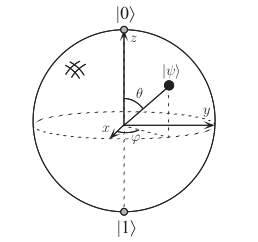
\includegraphics[scale = 0.5]{Images/bloch.png}}
\caption{Bloch sphere representation of a qubit}
\label{bloch}
\end{figure}

\subsection{Multiple qubits}
Suppose we have two qubits. If these were two classical bits, then there would be four
possible states, 00, 01, 10, and 11. Correspondingly, a two qubit system has four computational basis states 
\footnote{Another example of commonly used basis are called the ``bell states/EPR pairs'', given by $\ket{\beta_{00}} = \frac{\ket{00} + \ket{11}}{\sqrt{2}}; \ket{\beta_{01}} = \frac{\ket{01} + \ket{10}}{\sqrt{2}}; \ket{\beta_{10}} = \frac{\ket{00} - \ket{11}}{\sqrt{2}}; \ket{\beta_{11}} = \frac{\ket{01} - \ket{10}}{\sqrt{2}}$}
denoted $\ket{00}, \ket{10}, \ket{10}, \ket{11}$. A pair of qubits can also exist in
superpositions of these four states,
\begin{equation*}
    \ket{\psi} = \alpha_{00}\ket{00} + \alpha_{01}\ket{01} + \alpha_{10}\ket{10} + \alpha_{11}\ket{11}
\end{equation*}
Similar to the case for a single qubit, the measurement result x (= 00, 01, 10 or 11) occurs
with probability $|\alpha_x|^2$ , with the state of the qubits after the measurement being $\ket{x}$.
More generally, we may consider a system of n qubits. The computational basis states
of this system are of the form $\ket{x_{1}x_{2}{}_{\cdots}x_{n}}$, and so a quantum state of such a system
is specified by $2^n$ amplitudes.

\section{Quantum Gates}
Classical gates are responsible for manipulating bits, essentially representing a boolean function from bits to bits.
Similarly, quantum gates are just a function from qubits to qubits. In this section, we shall explore the different classes of quantum gates. 
We will not delve into proofs but offer an operational description of how quantum gates work. Further details for this can be found in \ref{gates}
\subsection{Single-Qubit gates}
A qubit can be written as a $2 \times 1$ unit vector in the space spanned by $\ket{0}, \ket{1}$. So, a transformation from a single qubit to 
another qubit transforms a unit vector to another unit vector. Hence, it follows that all quantum gates are unitary. Moreover, it turns out that any 
unitary operation is a valid quantum gate and can be constructed from some ``universal'' quantum gates (will be discussed later).

\begin{figure}[htbp]
\centerline{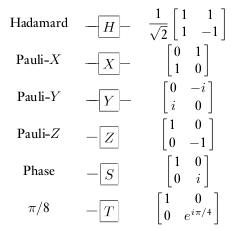
\includegraphics[scale = 0.5]{Images/single-gates.png}}
\caption{Single qubit gates}
\label{singlegate}
\end{figure}

Some single qubit quantum gates are shown in figure \ref{singlegate}. Since we are dealing with the qubit as an abstraction, a quantum gate is just a black box 
operator that performs a unitary transformation to a qubit. For now, we will not deal with the question of the physical realisation of these gates. 

\subsection{Multiple qubit gates}
In classical computation, there are five notable quantum gates, namely \verb|NOT|, \verb|AND|, \verb|OR|, \verb|NAND|, \verb|NOR|. As it turns out, 
all of these gates can be simulated using quantum gates as well. But, as a first step, consider the controlled-NOT, or the \verb|CNOT| gate (figure \ref{cnot}).
Now, we go into an important point when dealing with quantum gates. Even though the circuit diagram shows two input lines in the circuit, the \verb|CNOT| gate doesn't act on 
a single qubit, but a system of two ``entangled'' qubits. Hence, the only correct way to apply the circuit is to take the tensor product of the two input vectors, apply the gate and obtain 
another tensor product. The notation $\ket{a} \otimes \ket{b}$ is often abbreviated as $\ket{a}\ket{b}$ or $\ket{ab}$. So the action of a gate $U$ will be given as : 
\begin{equation*}
    \ket{a}\ket{b} \xrightarrow[]{U} U\ket{a}\ket{b}
\end{equation*}

\begin{figure}[htbp]
\centerline{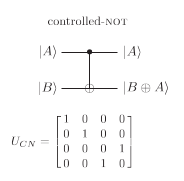
\includegraphics[scale = 0.7]{Images/cnot.png}}
\caption{CNOT gate}
\label{cnot}
\end{figure}

Moreover, just because the control qubit does not change values when it is a computational basis state doesn't mean that it will remain the same for all vectors. In fact, 
the control qubit often changes and measuring it's state is a key step in several quantum algorithms. Another important fact is that 
any multiple qubit quantum gate can be constructed using \verb|CNOT| and single qubit quantum gates. Hence, they form a set of universal quantum gates.
So, the \verb|CNOT| gate is analogous to the \verb|XOR| gate, but not exactly equivalent. Can gates be constructed exactly equivalent to \verb|NAND|, \verb|XOR| gates? Turns out this is 
not possible because quantum gates must be reversible whereas \verb|XOR| and \verb|NAND| gates are irreversible, i.e., given the output of these gates, the input cannot be uniquely identified. 

\subsection{Quantum circuits}
We have already seen some quantum circuits, but let us examine quantum ciruits in some more detail. Each line in the circuit is represented by a wire, but this wire is not necessarily physical, 
it may as well represent the passage of time, or a physical particle such as a photon. There are a few features allowed in classical circuits that are not usually present in
quantum circuits. Loops in a circuit are not allowed, \verb|FANOUT| and \verb|FANIN| operations are not allowed. This is because of the ``no-cloning''\footnote{The no-cloning theorem states that ``qubit-copying'' is not permitted. Hence, junctions of wires are not permitted in a quantum circuit. The no-cloning theorem proves to be useful in quantum encryption protocols like BB84 \cite{b4}} theorem.
An example of a quantum circuit is the ``quantum teleportation circuit''(figure \ref{teleport}). The setting of the problem is that Alice and Bob met long ago but now live
far apart. While together they generated an EPR pair, each taking one qubit of the EPR pair when they separated. Alice now wants deliver a qubit $\ket{\psi}$ to Bob. She does not know the state of
the qubit, and moreover can only send classical information to Bob. This can be achieved using the circuit given. 

\begin{figure}[htbp]
\centerline{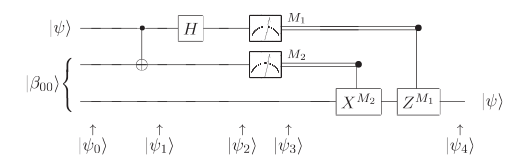
\includegraphics[scale = 0.5]{Images/teleport.png}}
\caption{Quantum circuit for teleporting a qubit. The two top lines represent Alice's system, while the bottom
line is Bob's system. The meters represent measurement, and the double lines coming out of them carry classical
bits (recall that single lines denote qubits)}
\label{teleport}
\end{figure}

\subsection{The Deutsch-Jozsa algorithm}
The problem is as follows. Alice, selects a number $x$ from $0$ to $2^n - 1$, and mails it in a letter to Bob. Bob calculates some function
$f(x)$ and replies with the result, which is either 0 or 1. Now, Bob has promised to use
a function $f$ which is of one of two kinds; either $f(x)$ is constant for all values of $x$,
or else $f(x)$ is balanced, that is, equal to 1 for exactly half of all the possible $x$, and 0
for the other half. Alice's goal is to determine with certainty whether Bob has chosen a
constant or a balanced function, corresponding with him as little as possible. In order to solve this we use the algorithm described (figure \ref{dj-algo}). 
The circuit for the same is shown in figure \ref{dj-ckt}
\begin{figure}[htbp]
\centerline{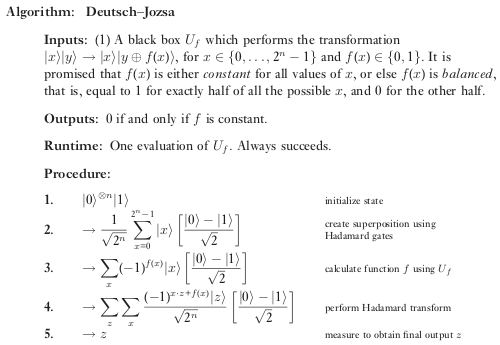
\includegraphics[scale = 0.5]{Images/deutch-algo.png}}
\caption{Deutsch-Jozsa algorithm}
\label{dj-algo}
\end{figure}

\begin{figure}[htbp]
\centerline{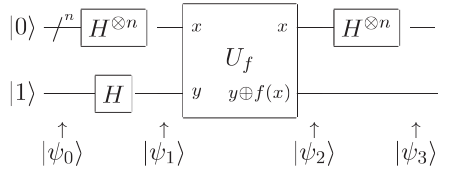
\includegraphics[scale = 0.5]{Images/deutch-ckt.png}}
\caption{Deutsch-Jozsa algorithm's circuit}
\label{dj-ckt}
\end{figure}

Finally, if the measurement yields all 0s then the function is constant, otherwise balanced. The reader can try verifying this as an exercise.

\section{The postulates of quantum mechanics}
Quantum mechanics is a mathematical framework for the development of physical theories. Just as newton's laws are axioms for classical mechanics, 
the postulates of quantum mechanics are not ``derived'', but assumed. The motivations of these postulates(axioms) may not always be clear, since 
they have been guessed after a lot of experimentation. So, this part of the report aims at knowing the postulates and gaining an operational understanding of the same. 
Understanding these axioms will  help us realise what happens in physical systems, and not the abstract vectors we have been dealing with till now.

\subsection{State space}
\textbf{Postulate 1} : Associated to any isolated physical system is a complex vector space
with inner product (that is, a Hilbert space) known as the state space of the
system. The system is completely described by its \textit{state vector}, which is a unit
vector in the system's state space.

Quantum mechanics does \textit{not} tell us, for a given physical system, what the state space
of that system is, nor does it tell us what the state vector of the system is. Figuring that
out for a specific system is a difficult problem for which physicists have developed many
intricate and beautiful rules. We will take the qubit as our fundamental quantum mechanical system.

\subsection{Evolution} \label{post2}
\textbf{Postulate 2} : The evolution of a \textit{closed} quantum system is described by a unitary
transformation. That is, the state $\ket{\psi}$ of the system at time $t_1$ is related to the
state $\ket{\psi}$ of the system at time $t_2$ by a unitary operator $U$ which depends only on
the times $t_1$ and $t_2$,
\begin{equation*}
    \ket{\psi^{'}} = U\ket{\psi}
\end{equation*}
Just as quantum mechanics does not tell us the state space or quantum state of a
particular quantum system, it does not tell us which unitary operators U describe real-world quantum dynamics. Quantum mechanics merely assures us that the evolution of
any closed quantum system may be described in such a way. Another interesting result follows from this postulate. If $t_1$
and $t_2$ are ``close'', then we can talk about derivative of functions, 

\textbf{Postulate 2'} : The time evolution of the state of a closed quantum system is
described by the Schrödinger equation
\begin{equation*}
    i\hbar\frac{d}{dt}\ket{\psi} = H\ket{\psi}
\end{equation*}
In this equation, $\hbar$ is a physical constant known as Planck's constant whose value
must be experimentally determined. The exact value is not important to us. In
practice, it is common to absorb the factor $\hbar$ into $H$, effectively setting $\hbar = 1$. $H$
is a fixed Hermitian operator known as the Hamiltonian of the closed system\footnote{Earlier, we spoke about applying a unitary operator to a system. Doesn't this contradict the fact that postulate 2 only holds for closed systems? Yes!
We should consider the experimentation set-up as a part of our system if we want to use the hamiltonian to describe it. But, the unitary operator is a good enough approximation
that we can push this nuance under the rug.}.

\subsection{Quantum measurement} \label{post3}
Even though the internal evolution of a quantum system can be worked out, there are times when we need to measure the quantum system, i.e. interact it with 
the experimental set-up which leads to the system not being closed anymore. This postulate addresses this development of the system. 

\textbf{Postulate 3} : Quantum measurements are described by a collection $\{M_m\}$ of
measurement operators. These are operators acting on the state space of the
system being measured. The index $m$ refers to the measurement outcomes that
may occur in the experiment. If the state of the quantum system is $\ket{psi}$
immediately before the measurement then the probability that result $m$ occurs is given by, 
\begin{equation*}
    p(m) = \bra{\psi}M_{m}^{\dag}M_{m}\ket{\psi}
\end{equation*}
and the state of the system after the measurement is
\begin{equation*}
    \frac{M_{m}\ket{\psi}}{\sqrt{\bra{\psi}M_{m}^{\dag}M_{m}\ket{\psi}}}
\end{equation*}
The measurement operators satisfy the completeness equation,
\begin{equation*}
    \sum_{m}M_{m}^{\dag}M_{m} = I
\end{equation*}
The completeness equation expresses the fact that probabilities sum to one:
\begin{equation*}
    1 = \sum_{m}p(m) = \sum_{m}\bra{\psi}M_{m}^{\dag}M_{m}\ket{\psi}
\end{equation*}

A simple but important example of a measurement is the measurement of a qubit in
the computational basis. This is a measurement on a single qubit with two outcomes
defined by the two measurement operators $M_0 = \ket{0}\bra{0}$, $M_1 = \ket{1}\bra{1}$. The probability of measured 
outcomes can be verified using this postulate.

An important application of Postulate 3 is to the problem of distinguishing quantum
states. In the classical world, distinct states of an object are usually distinguishable, at
least in principle. For example, we can always identify whether a coin has landed heads or
tails. An important result follows from postulate 3 that only only \textit{orthogonal states} can be distinguished.

\subsection{Composite systems}
\textbf{Postulate 4}: The state space of a composite physical system is the tensor product
of the state spaces of the component physical systems. Moreover, if we have
systems numbered $1$ through $n$, and system number $i$ is prepared in the state
$\ket{\psi_i}$, then the joint state of the total system is $\ket{\psi_1} \otimes \ket{\psi_2} \otimes \cdots \otimes \ket{\psi_n}$.

Further details about density operators, EPR can be found in \cite{b2}.

\section{Quantum circuits} \label{gates}
In this section, we will examine some more circuits and gates, theorems that help us to construct more complicated gates 
from simple building blocks.

The Pauli matrices give rise to three useful classes of unitary matrices when they are
exponentiated, the rotation operators about the $\hat{x}, \hat{y}$, and $\hat{z}$ axes, defined by the equations:
\begin{align*}
    R_{x}(\theta) \equiv e^{\frac{-i\theta X}{2}} &= cos\frac{\theta}{2}I - isin\frac{\theta}{2}X \\
    R_{y}(\theta) \equiv e^{\frac{-i\theta Y}{2}} &= cos\frac{\theta}{2}I - isin\frac{\theta}{2}Y \\
    R_{z}(\theta) \equiv e^{\frac{-i\theta Z}{2}} &= cos\frac{\theta}{2}I - isin\frac{\theta}{2}Z  
\end{align*}
\textit{Theorem} : (\textbf{Z-Y decomposition for a single qubit}) Suppose $U$ is a unitary
operation on a single qubit. Then there exist real numbers $\alpha, \beta, \gamma$ and $\delta$ such that
\begin{equation*}
    U = e^{i\alpha}R_{z}(\beta)R_{y}(\gamma)R_{x}(\delta)
\end{equation*}

\subsection{Controlled operation}
Suppose $U$ is an arbitrary single qubit unitary operation. A controlled-$U$ operation is a two qubit operation, again with a control and a target qubit. If the control
qubit is set then $U$ is applied to the target qubit, otherwise the target qubit is left alone; that is, 
\begin{equation*}
    \ket{c}\ket{t} \to \ket{c}U^{c}\ket{t}
\end{equation*}
where $\ket{c}, \ket{t}$ are computational basis states. The general operation is then done via tensor products.
The controlled-U operation is represented by the circuit shown in figure \ref{controlled-u}

\begin{figure}[htbp]
\centerline{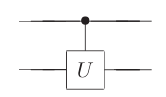
\includegraphics[scale = 0.5]{Images/controlled-u.png}}
\caption{Controlled-U operation. The top line is the control qubit, and the bottom line is the target qubit. If the
control qubit is set then U is applied to the target, otherwise it is left alone}
\label{controlled-u}
\end{figure}

Now, our goal is to construct a generalised controlled-U operation. In order to do this, the following theorem is useful : 

\textbf{Theorem} : Suppose $U$ is a unitary gate on a single qubit. Then there exist unitary
operators $A, B, C$ on a single qubit such that $ABC = I$ and $U = e^{i\alpha} AXBXC$,
where $\alpha$ is some overall phase factor.

First, let us consider the controlled phase shift operation. This operation does, $\ket{00} \to \ket{00}, \ket{01} \to \ket{01}, 
\ket{10} \to e^{i\alpha}\ket{10}, \ket{11} \to e^{i\alpha}\ket{11}$. The equivalent circuits for the same are given in figure \ref{controlled-phase-shift}

\begin{figure}[htbp]
\centerline{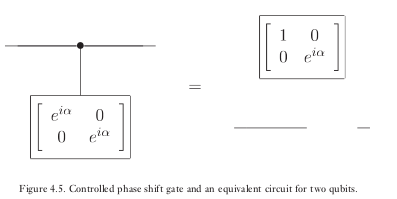
\includegraphics[scale = 0.5]{Images/controlled-phase-shift.png}}
\caption{Controlled phase shift gate and an equivalent circuit for two qubits}
\label{controlled-phase-shift}
\end{figure}

Now, we have enough to implement a controlled phase operation. The circuit for the same utilizes black boxes for $A, B, C$, and the \verb|CNOT| gate, along with 
controlled phase shift. The circuit is shown in figure \ref{u-exp}

\begin{figure}[htbp]
\centerline{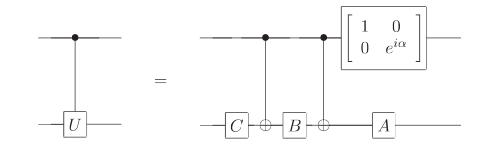
\includegraphics[scale = 0.5]{Images/u-exp.png}}
\caption{Circuit implementing the controlled-U operation for single qubit U}
\label{u-exp}
\end{figure}

\subsection{Multi-qubit controlled operations}

A well-known example of a multi-qubit control circuit is known as the \textit{toffoli gate}. 
This gate acts on the target qubit only if both the control qubits are in the $\ket{1}$ state. Hence, it is an extended 
\verb|CNOT| gate in some sense. 
The circuit for the same is shown in figure \ref{toffoli}

\begin{figure}[htbp]
\centerline{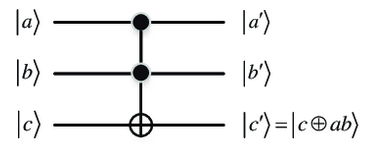
\includegraphics[scale = 0.5]{Images/toffoli.png}}
\caption{Toffoli gate}
\label{toffoli}
\end{figure}

We would further like to generalise this idea just as we did for a single control qubit. So, we introduce the generalised controlled-U gate, with 
$n$ control qubits and $k$ target qubits. This operator acts on a system of qubits as, 
\begin{equation*}
    C^{n}(U)\ket{x_{1}x_{2}{}_{\cdots}x_{n}}\ket{\psi} = \ket{x_{1}x_{2}{}_{\cdots}x_{n}}U^{x_{1}x_{2}{}_{\cdots}x_{n}}\ket{\psi}
\end{equation*}
where $x_{1}x_{2}{}_{\cdots}x_{n}$ in the exponent of $U$ means the product of the bits $x_{1}, x_{2},{}_{\cdots}, x_{n}$

\begin{figure}[htbp]
\centerline{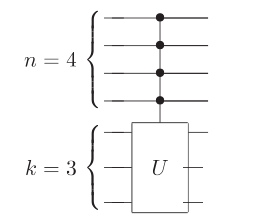
\includegraphics[scale = 0.5]{Images/gen_u_example.png}}
\caption{Sample circuit representation for the $C^{n}(U)$ operation, where $U$ is a unitary operator on $k$ qubits, for
$n = 4$ and $k = 3$.}
\label{gen-u-ex}
\end{figure}

Now, our task is to construct this generalised controlled-$U$ gate using the gates we know how to construct.
As it turns out, we can construct we can construct this gate using the single control qubit controlled-$U$ gate, and the toffoli gates. 
The circuit for the same has been shown in figure \ref{u-construct}.

\begin{figure}[htbp]
\centerline{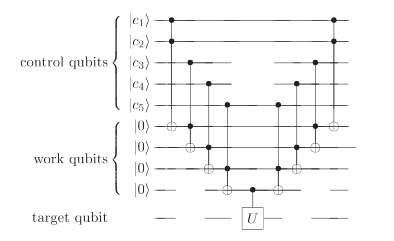
\includegraphics[scale = 0.5]{Images/u-construct.png}}
\caption{Network implementing the $C^{n}(U)$ operation, for the case $n = 5$.}
\label{u-construct}
\end{figure}

\subsection{Circuit Identities}
Here are some important circuit identities. Let subscripts denote which qubit an operator acts on, and let 
$C$ be a \verb|CNOT| with qubit $1$ the control qubit and qubit $2$ the target qubit. 
\begin{align*}
    CX_{1}C &= X_{1}X_{2} \\ 
    CY_{1}C &= Y_{1}X_{2} \\ 
    CZ_{1}C &= Z_{1} \\ 
    CX_{2}C &= X_{2} \\ 
    CY_{2}C &= Z_{1}Y_{2} \\
    CZ_{2}C &= Z_{1}Z_{2} \\
    R_{z,1}(\theta)C &= CR_{z,1}(\theta) \\ 
    R_{x,2}(\theta)C &= CR_{x,2}(\theta)
\end{align*} 

\subsection{Measurement \& Universal circuits}

There are really only two things worth knowing here : 
\begin{enumerate}
    \item The first principle is that classically conditioned operations 
    can be replaced by quantum conditioned operations
    \item \textbf{Principle of deferred measurement}: Measurements can always be moved from
    an intermediate stage of a quantum circuit to the end of the circuit; if the
    measurement results are used at any stage of the circuit then the classically
    controlled operations can be replaced by conditional quantum operations.
\end{enumerate}

Now, let's talk about universal quantum circuits. In classical circuits, \verb|NOT|, \verb|AND| and \verb|OR| are 
enough to describe any boolean function. Similarly for quantum circuits, there are three constructions we can make : 
\begin{enumerate}
    \item The first construction shows that an arbitrary unitary operator may be expressed ex-
    actly as a product of unitary operators that each acts non-trivially only on a subspace
    spanned by two computational basis states.
    \item The second construction combines the first
    construction with the results of the previous section to show that an arbitrary unitary
    operator may be expressed exactly using single qubit and \verb|CNOT| gates.
    \item The third construction combines the second construction with a proof that single qubit operation may
    be approximated to arbitrary accuracy using the Hadamard, phase, and $\pi/8$ gates.
\end{enumerate}

For more on universal quantum gates, one can refer \cite{b2}. 

\section{Quantum Fourier Transform}
The quantum Fourier transform is an efficient quantum algorithm for performing a Fourier transform of quantum mechanical amplitudes.
This idea is useful in algorithms like Grover's search. Let's explore the discrete fourier transform. Let $\ket{0}, \ket{1}, \cdots, \ket{N-1}$
be an orthonormal basis. Let the scalar coefficients corresponding to these basis states be $x_{1}, x_{2}, \cdots, x_{N-1}$. Then, the transformation is 
defined by; 
\begin{equation*}
    y_{k} \equiv \frac{1}{\sqrt{N}}\sum_{j=0}^{N-1}x_{j}e^{\frac{2\pi ijk}{N}}
\end{equation*}
\begin{equation*}
    \ket{j} \to \frac{1}{\sqrt{N}}\sum_{k=0}{N-1}e^{\frac{2\pi ijk}{N}}\ket{k}
\end{equation*}
Equivalently, an arbitrary state 
\begin{equation*}
    \sum_{j=0}^{N-1}x_{j}\ket{j} \xrightarrow{U} \sum_{k=0}^{N-1}y_{k}\ket{k}
\end{equation*}
where $U$ is a unitary operator. \\
In the following, we take $N = 2^n$ , where $n$ is some integer, and the basis $\ket{0}, \ket{1}, \cdots, \ket{2^n-1}$ is the 
computational basis for an $n$ qubit quantum computer. It is helpful to write the state 
$\ket{j}$ using the binary representation $j = j_{1}j_{2}{}_{\cdots}j_{n}$. 
More formally, $j = j_{1}2^{n-1} + j_{2}2^{n-2} + \cdots + j_{n}2^{0}$. It is also convenient to adopt the notation 
$0.j_{l}j_{l+1}{}_{\cdots}j_{m}$ to represent 
the binary fraction $j_{l}/2 + j_{l+1}/4 + \cdots + j_{m}/2^{m-l+1}$. 

With a little algebra the quantum Fourier transform can be given the following useful
\textit{product representation}:
\begin{equation*}
    \ket{j_{1}, {}_{\cdots}, j_{n}} \to \frac{(\ket{0} + e^{2\pi i0.j_{n}}\ket{1})\cdots(\ket{0} + e^{2\pi i0.j_{1}{}_{\cdots}j_{n-1}j_{n}}\ket{1})}{2^{n/2}}
\end{equation*}
This product representation is so useful that you may even wish to consider this to be the
definition of the quantum Fourier transform. This allows us to construct an efficient quantum circuit computing the Fourier transform, a
proof that the quantum Fourier transform is unitary, and provides insight into algorithms
based upon the quantum Fourier transform. \\ 
Let the gate $R_k$ denotes the unitary transformation; 
\begin{equation*}
    R_k \equiv 
    \begin{bmatrix}
    1 & 0 \\ 
    0 & e^{2\pi i/2^k}
    \end{bmatrix}
\end{equation*}
Given this, the quantum fourier transform circuit, i.e. an efficient algorithm for the same is shown in figure \ref{qft}.
\begin{figure}[htbp]
\centerline{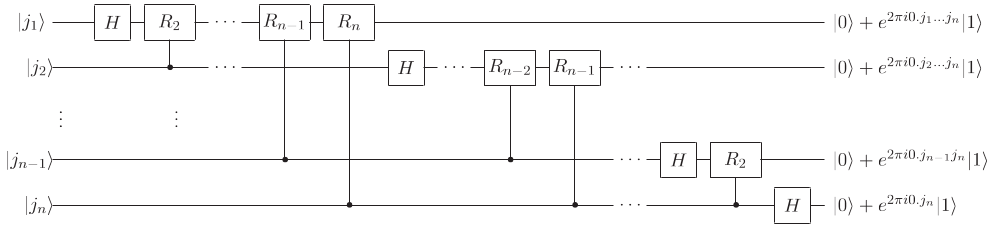
\includegraphics[scale = 0.25]{Images/qft.png}}
\caption{Efficient circuit for the quantum Fourier transform. This circuit is easily derived from the \textit{product
representation} for the quantum Fourier transform. Not shown are swap gates at the end of the circuit which
reverse the order of the qubits, or normalization factors of $1/\sqrt{2}$ in the output.}
\label{qft}
\end{figure}

\subsection{Phase estimation}
The Fourier transform is the key to a general procedure known as \textit{phase estimation},
which in turn is the key for many quantum algorithms. Suppose a unitary operator $U$
has an eigenvector $\ket{u}$ with eigenvalue $e^{2\pi i\phi}$, where the value of $\ket{\phi}$ is unknown. The goal
of the phase estimation algorithm is to estimate $\ket{\phi}$. To perform the estimation we assume
that we have available black boxes (sometimes known as oracles) capable of preparing the $j$
state $\ket{u}$ and performing the controlled-$U^{2^j}$ operation, for suitable non-negative integers
$j$.

The quantum phase estimation procedure uses two registers. The first register contains
$t$ qubits initially in the state $\ket{0}$. How we choose $t$ depends on two things: the number
of digits of accuracy we wish to have in our estimate for $\phi$, and with what probability
we wish the phase estimation procedure to be successful. 

The second register begins in the state $\ket{u}$, and contains as many qubits as is necessary
to store $\ket{u}$. Phase estimation is performed in two stages. First, we apply the circuit shown
in Figure \ref{phase-1}. 
\begin{figure}[htbp]
\centerline{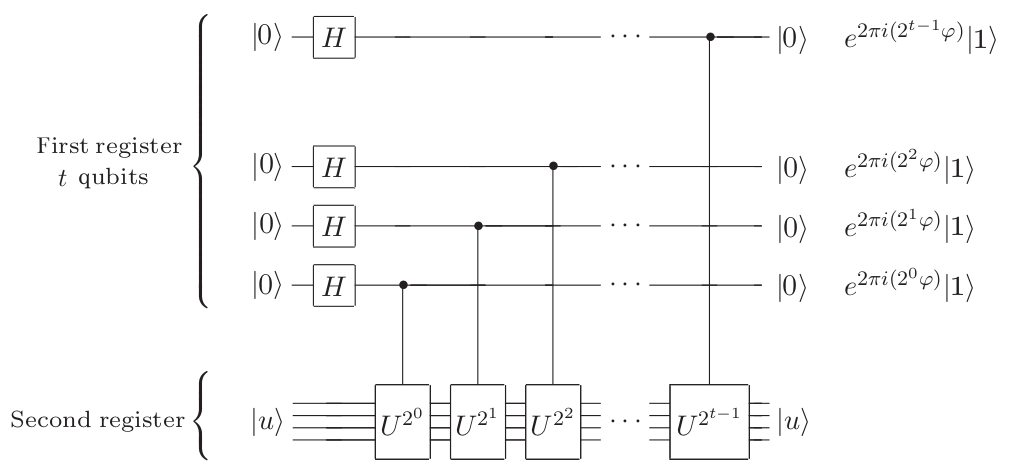
\includegraphics[scale = 0.25]{Images/phase-1.png}}
\caption{The first stage of the phase estimation procedure. Normalization factors of $1/\sqrt{2}$ have been omitted, on
the right.}
\label{phase-1}
\end{figure}
The second stage of phase estimation, shown in figure \ref{phase-2}, is to apply the inverse quantum Fourier transform
on the first register. This is obtained by reversing the circuit for the quantum Fourier
transform in the previous section, and can be done in $\Omega(t^2)$ steps. The
third and final stage of phase estimation is to read out the state of the first register by
doing a measurement in the computational basis.
\begin{figure}[htbp]
\centerline{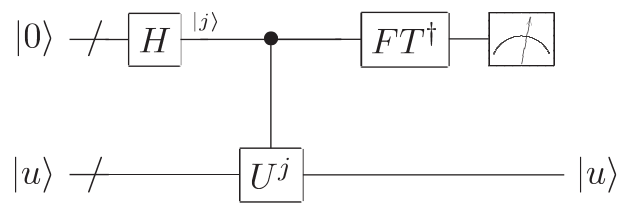
\includegraphics[scale = 0.25]{Images/phase-2.png}}
\caption{Schematic of the overall phase estimation procedure. The top $t$ qubits (the '/' denotes a bundle of
wires, as usual) are the first register, and the bottom qubits are the second register, numbering as many as required
to perform $U$. The state u is an eigenstate of $U$ with eigenvalue $e^{2i\pi\phi}$. The output of the measurement is an
approximation to $\phi$ accurate to $t - \ceil*{log(2 + \frac{1}{2\epsilon})}$ bits, with probability of success at least $1 - \epsilon$.}
\label{phase-2}
\end{figure}
Summarizing, the phase estimation algorithm allows one to estimate the phase $\phi$ of an
eigenvalue of a unitary operator $U$, given the corresponding eigenvector $\ket{u}$. An essential
feature at the heart of this procedure is the ability of the inverse Fourier transform to
perform the transformation
\begin{equation*}
    \frac{1}{2^{t/2}}\sum_{j=0}^{2^t-1}e^{2\pi i\phi j}\ket{j}\ket{u} \to \ket{\tilde{\phi}}\ket{u}
\end{equation*}
where $\tilde{\phi}$ denotes a state which is a good estimator for $\phi$ when measured.

\subsection{Application : Order finding}
As it turns out the problems of order finding and factoring are equivalent, that is, the problem of 
factoring can be expressed as an order finding problem. So, if we solve order finding, we get factoring for free.
Now, what is the order finding problem? For positive integers $x$ and $N$, $x < N$, with no common factors, the order of $x$ modulo $N$
is defined to be the least positive integer, $r$, such that $x^r \equiv 1$(mod $N$).

The quantum algorithm for order-finding is just the phase estimation algorithm applied
to the unitary operator
\begin{equation*}
    U\ket{y} = \ket{xy(\text{mod N})}
\end{equation*}
with $y \in \{0, 1\}^L$. (Note that here and below, when $N \leq y \leq 2^L - 1$, we use the
convention that $xy$(mod N) is just $y$ again. That is, $U$ only acts non-trivially when
$0 \leq y \leq N - 1$). A simple calculation shows that the states defined by
\begin{equation*}
    \ket{u_s} \equiv \frac{1}{\sqrt{r}}\sum_{k=0}^{r-1}e^{-\frac{2\pi isk}{r}\ket{x^k \text{ mod N}}}
\end{equation*}
for integer $0 \leq s \leq r - 1$ are eigenstates of $U$ , since
\begin{align*}
    U\ket{u_s} &= \frac{1}{\sqrt{r}}\sum_{k=0}^{r-1}e^{-\frac{2\pi isk}{r}\ket{x^{k+1} \text{ mod N}}} \\ 
    &= e^{\frac{2\pi is}{r}}\ket{u_s}
\end{align*}
Using the phase estimation procedure allows us to obtain, with high accuracy, the corresponding 
eigenvalues $exp(2\pi is/r)$, from which we can obtain the order $r$ with a little bit more work.

There are two important requirements for us to be able to use the phase estimation
procedure: we must have efficient procedures to implement a controlled-$U^{2^j}$ operation
for any integer $j$, and we must be able to efficiently prepare an eigenstate $\ket{u_s}$ with a non-trivial 
eigenvalue, or at least a superposition of such eigenstates. The first requirement
is satisfied by using a procedure known as modular exponentiation, with which we
can implement the entire sequence of controlled-$U^{2^j}$ operations applied by the phase
estimation procedure using $O(L^3)$ gates. \\ 
The second requirement is a bit trickier. preparing $\ket{u_s}$ requires that we know $r$, so
this is out of the question. Fortunately, there is a clever observation which allows us to
circumvent the problem of preparing $\ket{u_s}$, which is that : 
\begin{equation*}
    \frac{1}{\sqrt{r}}\sum_{s=0}^{r-1}\ket{u_s} = \ket{1}
\end{equation*}
Hence, preparing $\ket{1}$ in the second register suffices, which is trivial. Hence, the circuit is complete and is shown in 
figure \ref{order}

\begin{figure}[htbp]
\centerline{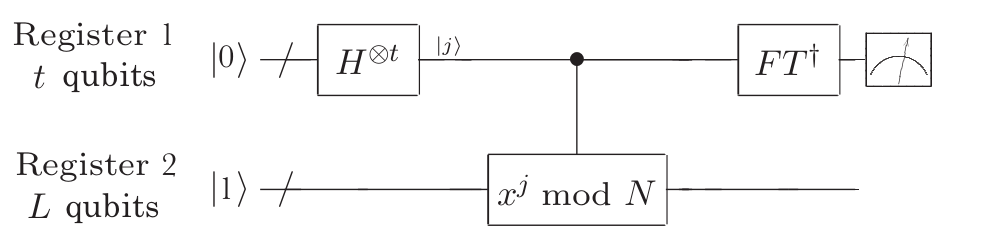
\includegraphics[scale = 0.25]{Images/order.png}}
\caption{Quantum circuit for the order-finding algorithm.}
\label{order}
\end{figure}

Even after doing this, we are not done yet. The measurement will give us an estimate of $s/r$. We need to determine the value of $r$ from this. This can be done using the continued fractions 
expansion since we know the number of bits upto which these numbers upto a good accuracy. The process of continued fractions finally yields us $r$.
The algorithm has been summarised in figure \ref{order-summ}

\begin{figure}[htbp]
\centerline{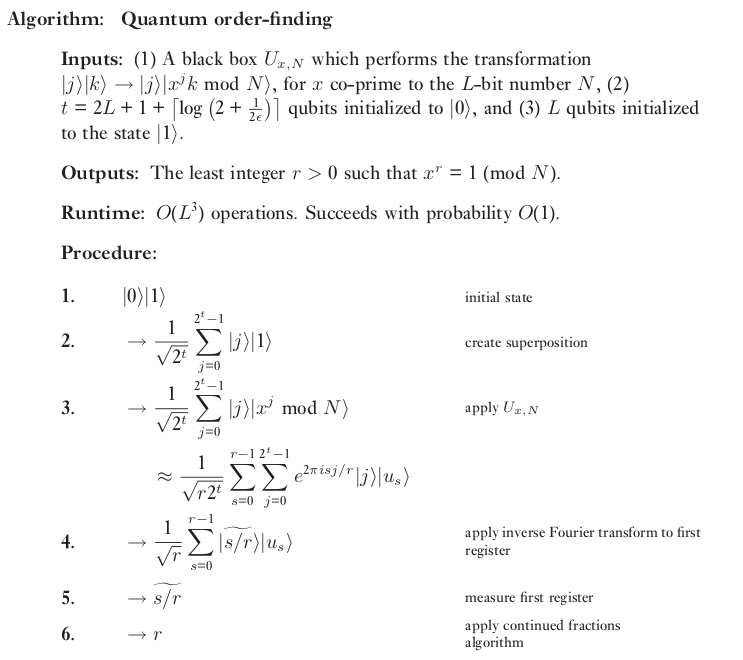
\includegraphics[scale = 0.3]{Images/order-summary.png}}
\caption{Algorithm for the order-finding problem}
\label{order-summ}
\end{figure}

\subsection{Application : Factoring}
The factoring problem is given a natural number $N \in \N$, to return a non-trivial factor of $N$, that is, other than 1 and $N$ itself.
As described earlier, we will simply reduce this problem into order-finding. This is how we do it. 
\begin{enumerate}
    \item If $N$ is even, return the factor $2$.
    \item Determine whether $N = a^b$ for integers $a \geq 1$ and $b \geq 2$, and if so
    return the factor $a$ (classical algorithm described in \cite{b6}).
    \item Randomly choose $x$ in the range $1$ to $N-1$. If $gcd(x, N) > 1$ then return
    the factor $gcd(x, N)$.
    \item Use the order-finding subroutine to find the order $r$ of $x$ modulo $N$ .
    \item If $r$ is even and $x^{r/2} \neq - 1(\text{mod N})$ then compute $gcd(x^{r/2} - 1, N)$ and
    $gcd(x^{r/2} + 1, N)$, and test to see if one of these is a non-trivial factor,
    returning that factor if so. Otherwise, the algorithm fails.
\end{enumerate}
That is it. 

\section{Quantum Search Algorithms}

To be completed.

\section*{Acknowledgement}
I would like to thank the mentors of this project Siddhant Midha and Aditya Sriram for giving 
me the opportunity to study and appreciate this subject. 

\begin{thebibliography}{00}
\bibitem{b1} M. Schuld, I. Sinayskiy and F. Petruccione, ``An introduction to quantum machine learning,'' September 2014.
\bibitem{b2} M. Neilson and I. Chuang, ``Quantum Computing and Quantum Information, 10\textsuperscript{th} edition''
\bibitem{b3} S. Midha and A. Sriram ``Learning with Quantum Computers'' \href{https://github.com/siddhant-midha/WiDS-22-Learning-with-quantum-computers-}{\textit{Github repository}}, January 2023.
\bibitem{b4} C. H. Bennett, G. Brassard ``Quantum cryptography: Public key distribution and coin tossing'' March 2020.
\bibitem{b5} O. Simeone ``An Introduction to Quantum Machine Learning for Engineers'' May 2022.
\bibitem{b6} D. J. Bernstein. \href{http://cr.yp.to/papers/powers-19971106-retypeset20220326.pdf}{``Detecting perfect powers in essentially linear time"}. Mathematics of Computation 67 (1998), 1253-1283 Date: 1997.11.06. AMS version: 31pp.
\end{thebibliography}
\vspace{12pt}

\end{document}
